\documentclass[conference]{IEEEtran}

\usepackage[utf8]{inputenc}
\usepackage[T5]{fontenc}
\usepackage{cite}
\usepackage{amsmath,amssymb,amsfonts}
\usepackage{graphicx}
\usepackage{textcomp}
\usepackage{xcolor}
\usepackage{booktabs}
\usepackage{multirow}
\usepackage{url}
\usepackage{float}
\usepackage{xurl}

\begin{document}

\title{A Unified Subject-Wise Evaluation of CNN, RNN, Transformer, and State Space Architectures for Single-Channel EEG Sleep Staging}

\author{
\IEEEauthorblockN{
\textsuperscript{} Nguyen Viet Hung,
\textsuperscript{} Le Duc Gia Bao,
\textsuperscript{} Huynh Quang Tri, and
\textsuperscript{} Vu Nguyen Minh Long
}
\IEEEauthorblockA{
\textit{Artificial Intelligence Department}\\
\textit{FPT University}\\
Ho Chi Minh City, Vietnam\\
\{hung2272006, giabao240806, huynhquangtri35, vunguyenminhlong485\}@gmail.com
}
}

\maketitle

\begin{abstract}
Automatic sleep staging can reduce the workload associated with manual interpretation of overnight polysomnography, but comparisons among deep learning systems are often confounded by differences in preprocessing, subject partitioning, sequence construction, optimization, and metric implementation. This work presents a unified subject-wise benchmark of adapted deep learning architectures, covering CNN-based, CNN-RNN, Transformer-based, and State Space approaches for single-channel EEG sleep staging. All architectures were reimplemented under a common experimental framework rather than directly reproduced from their original implementations. Specifically, we evaluate adapted implementations inspired by TinySleepNet, DeepSleepNet, SleepTransformer, and Mamba-based state-space architectures. Experiments used 153 Sleep Cassette recordings from the Sleep-EDF Expanded database. The Fpz--Cz EEG channel was divided into 30-s epochs, mapped to five stages, and normalized independently by epoch. All models were evaluated using the same subject-wise 10-fold protocol, recording-safe sequence construction, weighted cross-entropy, checkpoint rule, and masked metrics. Among the evaluated models, TinySleepNet-adapted achieved a macro-F1 of $0.7439\pm0.0322$, while DeepSleepNet-adapted obtained $0.6823\pm0.0457$ macro-F1. SleepTransformer-adapted obtained the highest observed mean accuracy, macro-F1, and Cohen's kappa: $0.8951\pm0.0151$, $0.7522\pm0.0273$, and $0.7940\pm0.0281$, respectively. MambaSleep-adapted achieved $0.7091\pm0.0304$ macro-F1, exceeding the DeepSleepNet-adapted implementation. N1 remained the most difficult stage for every model even though N3 was less frequent. An exploratory paired fold-level analysis indicated a statistically significant accuracy difference between SleepTransformer-adapted and TinySleepNet-adapted after Holm correction, whereas their macro-F1 and Cohen's kappa differences did not reach the corrected threshold. The results emphasize the importance of subject-wise evaluation and careful distinction between original published architectures and repository-specific adaptations.
\end{abstract}

\begin{IEEEkeywords}
automatic sleep staging, electroencephalography, Sleep-EDF Expanded, subject-wise cross-validation, deep learning, CNN-RNN, Transformer, State Space Model
\end{IEEEkeywords}

\section{Introduction}

Sleep staging is a central component of clinical sleep assessment. Overnight polysomnography records physiological signals such as electroencephalography (EEG), electrooculography, electromyography, and electrocardiography. The recording is conventionally divided into 30-s epochs and each epoch is assigned to a sleep stage. Manual scoring is labor-intensive and is affected by inter-scorer variability, which has motivated extensive research on automatic sleep-staging systems.

Public datasets such as Sleep-EDF have supported the development and comparison of data-driven approaches \cite{sleepedfx_dataset,kemp2000analysis}. Traditional systems commonly combine hand-crafted temporal, spectral, entropy, or time--frequency features with a conventional classifier. Such pipelines remain relevant because they can be interpretable and competitive when carefully designed \cite{vandonckt2023traditional,lal2023temporal}. Nevertheless, deep neural networks reduce dependence on manual feature engineering and can jointly learn local EEG morphology and temporal context.

Convolutional recurrent architectures have played a major role in this development. DeepSleepNet combines parallel convolutional branches with bidirectional recurrent modeling \cite{supratak2017deepsleepnet}, while TinySleepNet uses a more compact CNN--LSTM design \cite{supratak2020tinysleepnet}. Sequence-to-sequence methods such as SeqSleepNet explicitly predict all stages in an input context \cite{phan2019seqsleepnet}. Other studies have explored joint classification and neighboring-stage prediction \cite{phan2018joint}, fully convolutional segmentation \cite{perslev2019utime}, and hybrid CNN--LSTM architectures \cite{li2023hybrid,toma2023multichannel}.

Attention-based models provide a different mechanism for temporal interaction. The Transformer introduced self-attention as an alternative to recurrence \cite{vaswani2017attention}. AttentionSleepNet and SleepTransformer adapted attention mechanisms to sleep staging \cite{eldele2021attention,phan2022sleeptransformer}. Multi-view and multimodal models have additionally combined raw signals, spectral representations, or several physiological channels \cite{phan2022xsleepnet,zheng2022mmasleepnet}. More recently, selective state-space models such as Mamba have been proposed for efficient sequence processing \cite{gu2023mamba}, and WaveMamba combined wavelet decomposition with state-space modeling for full-night sleep staging \cite{sano2025wavemamba}.

Despite this progress, published performance values are difficult to compare directly. Studies differ in dataset subset, EEG derivation, wake trimming, normalization, context length, split policy, optimization, and metric calculation. Subject leakage is especially problematic because multiple recordings from one participant can be assigned to different subsets. Moreover, the fidelity of open-source reimplementations to their corresponding papers can vary. A controlled benchmark must therefore define both the shared protocol and the exact repository implementations being compared.

We provide a unified implementation and subject-wise evaluation framework for four representative deep learning architectures, including CNN-based, CNN-RNN, Transformer-based, and State Space Model approaches. All four architectures were reimplemented within a unified PyTorch framework. TinySleepNet-adapted primarily preserves the original architectural design with framework-level modifications, while the remaining architectures required additional architectural adaptations to support the proposed single-channel EEG setting.

The contributions are:
\begin{itemize}
    \item a subject-wise 10-fold benchmark in which all recordings from one participant remain in the same fold;
    \item a preprocessing description grounded in the original notebook used to create the NPZ corpus;
    \item a shared many-to-many training and evaluation pipeline with recording-safe windows and masked padded positions;
    \item overall, class-wise, cross-fold variation, and paired statistical analyses of the four adapted architectures; and
    \item an explicit separation between original published architectures and our adapted implementations.
\end{itemize}

\section{Related Work}

\subsection{Convolutional and Recurrent Sleep-Staging Models}

DeepSleepNet demonstrated end-to-end sleep staging from raw single-channel EEG using two convolutional branches and bidirectional LSTM layers \cite{supratak2017deepsleepnet}. TinySleepNet reduced architectural complexity through a single convolutional branch and a unidirectional LSTM while retaining sequence modeling and class-aware training \cite{supratak2020tinysleepnet}. SeqSleepNet framed sleep staging as hierarchical many-to-many prediction, with an epoch-level encoder and a sequence-level recurrent network \cite{phan2019seqsleepnet}. A related framework jointly classified the current epoch and predicted neighboring stages to improve contextual representation learning \cite{phan2018joint}.

Fully convolutional alternatives have also been studied. U-Time used an encoder--decoder architecture for dense time-series segmentation \cite{perslev2019utime}. Hybrid systems have combined deep residual feature extraction, squeeze-and-excitation, and LSTM modeling for single-channel EEG \cite{li2023hybrid}; multi-channel CNN--BiLSTM networks have been used when several physiological signals are available \cite{toma2023multichannel}. Evaluation in clinical populations with suspected obstructive sleep apnea further showed the need to assess robustness outside highly curated cohorts \cite{korkalainen2019clinical}.

\subsection{Multi-View, Transfer, and Self-Supervised Learning}

Sleep-stage information can be represented as raw waveforms, spectral features, or several physiological modalities. XSleepNet jointly learned from raw and time--frequency views and used gradient blending to balance their contributions \cite{phan2022xsleepnet}. MMASleepNet used multimodal attention to integrate electrophysiological signals \cite{zheng2022mmasleepnet}. These approaches can exploit complementary information but require more complex inputs than the single-channel setting considered here.

Generalization across subjects and datasets remains difficult. Personalized adaptation with single-night data has been explored using Kullback--Leibler regularization \cite{phan2020personalized}. Deep transfer learning and unsupervised domain adaptation have been proposed to reduce performance degradation across datasets and recording conditions \cite{phan2020transfer,fan2022domain}. Cross-domain transfer among EEG and ECG tasks further illustrates the potential and limitations of reusing physiological representations \cite{yang2023cross}. Self-supervised learning offers another route to label efficiency by exploiting unlabeled sleep recordings before supervised fine-tuning \cite{eldele2023selfsupervised}.

\subsection{Attention, Explainability, and Class Imbalance}

The Transformer architecture established self-attention as a general sequence-modeling mechanism \cite{vaswani2017attention}. In sleep staging, attention has been applied both within epochs and across temporal context \cite{eldele2021attention,phan2022sleeptransformer}. Lightweight segmented attention networks fuse local characteristics with adjacent information \cite{zhou2022lightweight}, while parallel frequency-cut attention models interactions among time--frequency regions \cite{chen2023frequencycut}. Self-attention and Gaussian-noise augmentation have also been evaluated in pediatric sleep staging \cite{huang2023children}.

Attention weights and post-hoc explanation methods have been used to improve model transparency. SleepTransformer investigated interpretability and uncertainty in addition to classification \cite{phan2022sleeptransformer}, and SleepXAI combined deep sleep-stage prediction with explainability techniques \cite{dutt2023sleepxai}. These capabilities belong to the original studies; they are not evaluated by the raw-EEG SleepTransformer-adapted implementation in this benchmark.

Class imbalance remains an important challenge, particularly for transitional N1 epochs. Work on augmentation, generative methods, and class-aware network design has attempted to improve minority-stage performance \cite{zhou2022imbalance}. Traditional machine-learning studies also show that strong feature engineering can remain competitive and may offer better transparency \cite{vandonckt2023traditional,lal2023temporal}.

\subsection{State-Space and Wavelet Models}

Selective state-space models provide an alternative to recurrent networks and quadratic self-attention. Mamba makes state-space parameters input dependent so that the model can selectively propagate or forget information \cite{gu2023mamba}. WaveMamba combines multi-resolution wavelet features with state-space blocks for full-night sleep staging \cite{sano2025wavemamba}. MambaSleep-adapted is evaluated as a lightweight state-space architecture. It utilizes fixed wavelet decomposition, frequency-specific branches, cross-band attention, and Mamba-inspired temporal updates.

\section{Materials and Methods}

\subsection{Dataset}

Experiments used the Sleep Cassette subset of the Sleep-EDF Database Expanded \cite{sleepedfx_dataset,kemp2000analysis}. The corpus contains 153 overnight recordings from 78 participants, with most participants contributing two nights. Only the Fpz--Cz EEG derivation was used.

The evaluated NPZ corpus contains 414,961 retained epochs. Table~\ref{tab:distribution} shows the class distribution. Wake is dominant because the notebook preserves the available wake periods rather than applying a pre/post-sleep wake-trimming rule. N3 is the least frequent class, whereas N1 is the second least frequent.
% \begin{figure}
%     \centering
%     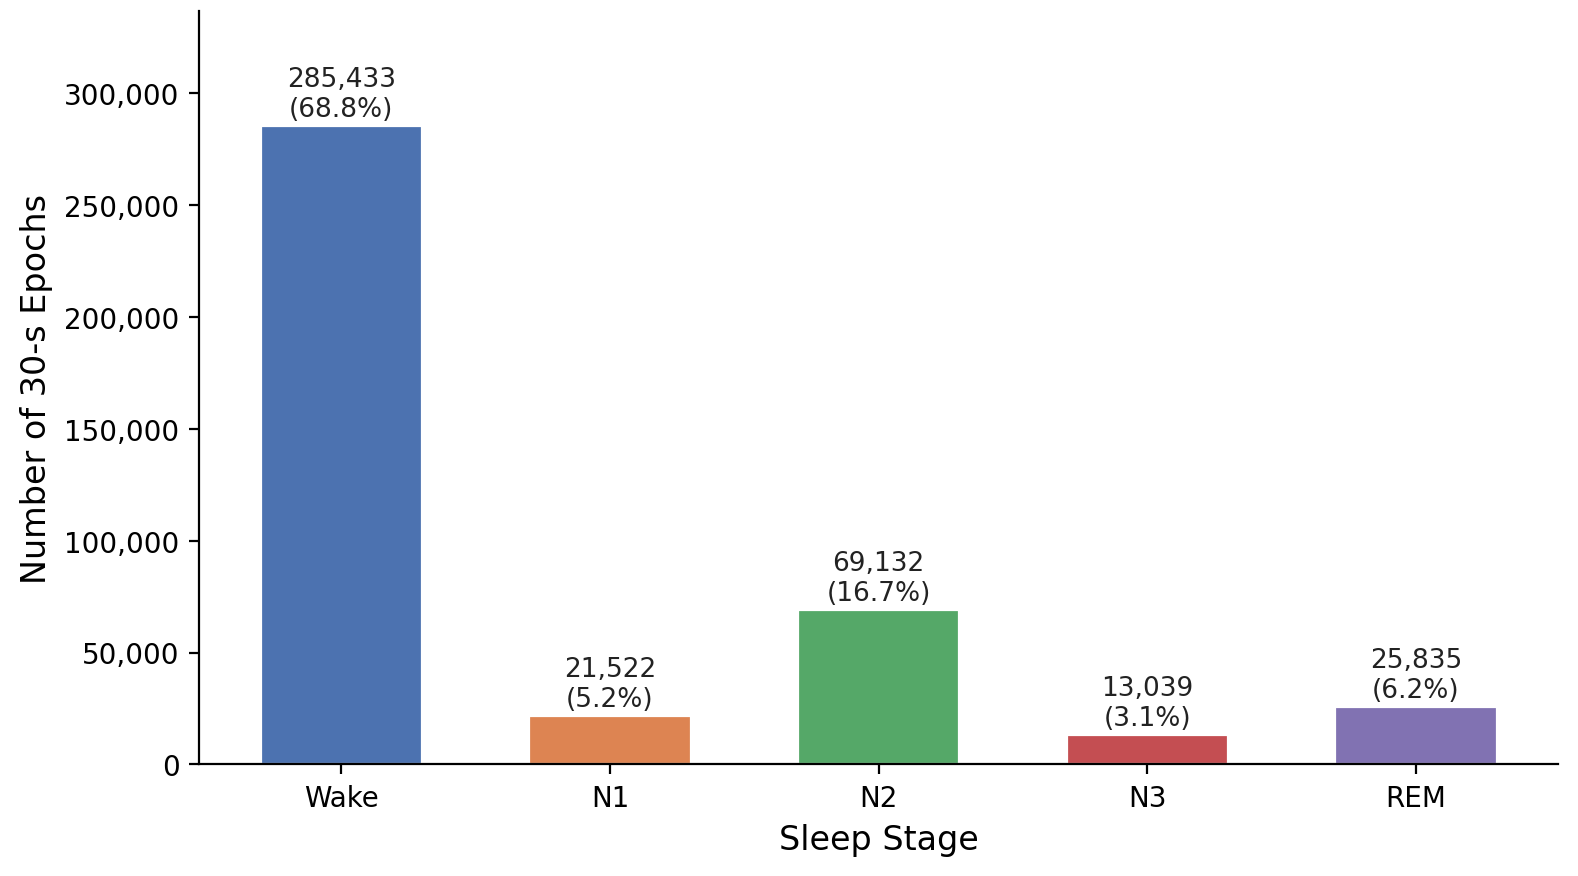
\includegraphics[width=1\linewidth]{fig3_class_distribution.png}
%     \caption{\textbf{Class Distribution of the Evaluated Corpus}}
%     \label{fig:placeholder}
% \end{figure}
\begin{table}[H]
\centering
\caption{Class Distribution of the Evaluated Corpus}
\label{tab:distribution}
\begin{tabular}{lrr}
\toprule
Stage & Epochs & Percentage \\
\midrule
W   & 285,433 & 68.79\% \\
N1  & 21,522  & 5.19\% \\
N2  & 69,132  & 16.66\% \\
N3  & 13,039  & 3.14\% \\
REM & 25,835  & 6.23\% \\
\midrule
Total & 414,961 & 100.00\% \\
\bottomrule
\end{tabular}
\end{table}

\subsection{EEG Preprocessing}

The preprocessing notebook uses MNE-Python to read PSG EDF files and their corresponding hypnogram annotations \cite{gramfort2014mne}. For the benchmark corpus, the Fpz--Cz channel is selected. Sleep annotations are converted into 30-s events using the following mapping:
\begin{equation}
\mathrm{W}\rightarrow0,\quad
\mathrm{S1}\rightarrow1,\quad
\mathrm{S2}\rightarrow2,\quad
\mathrm{S3/S4}\rightarrow3,\quad
\mathrm{REM}\rightarrow4.
\end{equation}
Annotations outside these five targets are not included in the event map and therefore are not extracted as training epochs.

The Sleep Cassette EEG is sampled at 100 Hz, so each 30-s epoch contains 3000 samples. MNE epochs are created with $t_{\min}=0$ and
\begin{equation}
t_{\max}=30-\frac{1}{f_s}.
\end{equation}
No baseline correction is applied. Each epoch is standardized independently along the sample dimension:
\begin{equation}
\widetilde{x}_{i}(t)=
\frac{x_i(t)-\mu_i}{\sigma_i+10^{-7}},
\end{equation}
where $\mu_i$ and $\sigma_i$ are the mean and standard deviation of epoch $i$. The notebook does not apply an additional band-pass filter, resampling operation, or wake trimming in the Fpz--Cz extraction path used for this benchmark. Each recording is stored as one NPZ file containing \texttt{x} with shape $(N,1,3000)$ and \texttt{y} with shape $(N,)$.

\subsection{Subject-Wise Cross-Validation}

Recording names such as \texttt{SC4001} and \texttt{SC4002} share the first five characters and are therefore assigned to the same subject identifier. The 78 unique subjects are shuffled with seed 42 and partitioned into ten folds. For experiment $i$, fold $i$ is the test set, fold $(i+1)\bmod10$ is the validation set, and the remaining eight folds form the training set:
\begin{align}
\mathcal{D}^{(i)}_{\mathrm{test}} &= \mathcal{F}_{i},\\
\mathcal{D}^{(i)}_{\mathrm{val}} &= \mathcal{F}_{(i+1)\bmod 10},\\
\mathcal{D}^{(i)}_{\mathrm{train}} &=
\bigcup_{j\notin\{i,(i+1)\bmod10\}}\mathcal{F}_{j}.
\end{align}
Before training, the implementation asserts that the train, validation, and test subject sets are pairwise disjoint.

\subsection{Sequence Construction and Augmentation}

All models perform many-to-many prediction over sequences of $L=20$ epochs:
\begin{equation}
\mathbf{X}\in\mathbb{R}^{B\times20\times1\times3000},
\qquad
\mathbf{Y}\in\{0,\ldots,4\}^{B\times20}.
\end{equation}
Windows are created independently inside each recording; epochs from different nights are never concatenated.

Training windows use stride 5 and only complete sequences are retained. Two train-only augmentations are applied once when the dataset object is constructed. First, all epochs in a recording receive the same random temporal shift from $-300$ to $299$ samples, using zero padding rather than circular wrapping. Second, zero to four initial epochs are skipped before window generation. Validation and test windows use stride 20. A final incomplete window is zero-padded, and a binary mask identifies valid positions. Padded positions are excluded from both the loss and evaluation metrics.

\subsection{Model Adaptation and Unified Implementation}

Although inspired by previous sleep staging architectures, all models were reimplemented under a unified PyTorch framework. The objective of these adaptations is to enable fair comparison under a common experimental setting rather than to reproduce the original implementations exactly. All adaptations were designed to maintain comparable evaluation conditions across architectures.

Specifically, the original designs were adapted to the following unified pipeline:
\begin{itemize}
    \item \textbf{Single-channel EEG input:} All models receive the single-channel Fpz--Cz EEG derivation as their raw input.
    \item \textbf{Identical preprocessing pipeline:} Every model uses the same independent epoch-wise Z-score standardization.
    \item \textbf{Unified sequence length:} The models operate on sequence contexts of $L=20$ epochs.
    \item \textbf{Subject-wise cross-validation protocol:} All architectures are evaluated using the identical subject-wise 10-fold scheme.
    \item \textbf{Consistent optimization and training strategy:} Every model is trained with the same AdamW optimizer, weight decay, masked weighted cross-entropy loss, and validation-based early stopping.
\end{itemize}
Therefore, the evaluated systems should be interpreted as adapted implementations rather than exact reproductions of the original publications.

\subsection{Evaluated Architectures}

\begin{table*}[t]
\centering
\caption{Architectures Used in the Unified Benchmark}
\label{tab:models}
\begin{tabular}{p{2.6cm}p{4.0cm}p{3.6cm}p{5.4cm}}
\toprule
Model & Epoch representation & Temporal module & Relation to the original work \\
\midrule
TinySleepNet-adapted &
Single CNN branch producing a 2048-dimensional epoch vector &
One-layer unidirectional LSTM with 128 hidden units &
PyTorch adaptation inspired by \cite{supratak2020tinysleepnet} integrated into the common many-to-many interface \\
DeepSleepNet-adapted &
Parallel small- and large-filter CNN branches followed by a 512-dimensional projection &
Two-layer bidirectional LSTM with 256 units per direction and a residual shortcut &
DeepSleepNet-style architecture trained end-to-end in one stage; inspired by \cite{supratak2017deepsleepnet} but does not reproduce the original two-stage optimization \\
SleepTransformer-adapted &
CNN front-end producing 29 frame tokens of dimension 128; two intra-epoch Transformer layers and attention pooling &
Two inter-epoch Transformer encoder layers &
Raw-EEG SleepTransformer-style adaptation inspired by \cite{phan2022sleeptransformer} rather than an exact reproduction of the original input pipeline \\
MambaSleep-adapted &
Four-level fixed db4 decomposition, five lightweight CNN branches, and four-head cross-band attention &
Two compact pure-PyTorch Mamba-inspired temporal blocks &
Lightweight state-space adapted implementation inspired by Mamba principles \cite{gu2023mamba}, operating on 20 epochs rather than full-night context \\
\bottomrule
\end{tabular}
\end{table*}

TinySleepNet-adapted primarily preserves the compact CNN--LSTM design of the original TinySleepNet architecture \cite{supratak2020tinysleepnet}. Its CNN produces a 2048-dimensional representation for each epoch, and a unidirectional LSTM produces contextual features for per-epoch classification.

The DeepSleepNet-adapted architecture is inspired by the dual-receptive-field concept of the original DeepSleepNet model \cite{supratak2017deepsleepnet}. The small branch begins with kernel size 50 and stride 6, whereas the large branch begins with kernel size 400 and stride 50. Their outputs are projected to 512 dimensions and processed by a bidirectional LSTM.

The SleepTransformer-adapted implementation is inspired by the Transformer family \cite{vaswani2017attention,phan2022sleeptransformer} and uses a CNN to generate 29 frame-level tokens. Two eight-head Transformer layers model intra-epoch structure, learnable attention pooling produces epoch vectors, and two additional Transformer layers model the 20-epoch sequence. The general self-attention mechanism follows the original architecture, but the raw-EEG CNN front-end differs from the original SleepTransformer pipeline \cite{phan2022sleeptransformer}.

MambaSleep-adapted decomposes each epoch into $A_4,D_4,D_3,D_2,$ and $D_1$ using fixed Daubechies-4 filters. Five lightweight CNN branches produce 96-dimensional band tokens. Cross-band attention fuses these tokens, and two Mamba-inspired blocks model the epoch sequence. The design of MambaSleep-adapted is motivated by state-space modeling principles \cite{gu2023mamba}, while introducing a lightweight computational structure that avoids expensive Mamba stacks in the frequency branches.

\subsection{Training Protocol}

Every model is trained for at most 50 epochs with batch size 32. AdamW is used with learning rate $10^{-4}$ and weight decay $10^{-4}$ \cite{loshchilov2017adamw}. Gradients are clipped to a maximum norm of 5.0. Python, NumPy, and PyTorch random generators use seed 42, with deterministic cuDNN behavior enabled.

Class weights are computed only from the current training files:
\begin{equation}
w_c=\frac{N}{5N_c+\epsilon},
\end{equation}
where $N_c$ is the number of training epochs belonging to class $c$. The masked weighted cross-entropy is
\begin{equation}
\mathcal{L}=
-\frac{\sum_{(b,t)\in\Omega} w_{y_{b,t}}\log p_{b,t,y_{b,t}}}
      {\sum_{(b,t)\in\Omega} w_{y_{b,t}}}
\end{equation}
where $\Omega$ contains valid, non-padded positions. The checkpoint with the highest validation macro-F1 is retained. Training stops after 15 consecutive epochs without validation macro-F1 improvement.

\subsection{Evaluation and Statistical Analysis}

Accuracy, macro-F1, per-class F1, and Cohen's kappa are calculated after removing padded positions. Cohen's kappa measures agreement beyond chance \cite{cohen1960coefficient}. Macro-F1 is calculated over the fixed label set $\{0,1,2,3,4\}$, and an undefined class F1 is assigned zero. All ten test folds contained at least one valid epoch from each of the five sleep stages. Therefore, no class-wise F1 value was undefined because of an entirely absent test class. The fixed label set and zero-division rule were nevertheless retained to ensure consistent metric computation.

The repository summary reports the mean and NumPy population standard deviation across the ten test folds. In addition, this study performs an exploratory Friedman test across the four paired model results for each overall metric. When the global test indicates differences, exploratory two-sided exact Wilcoxon signed-rank tests are performed for all six model pairs, followed by Holm correction within each metric. The nominal significance threshold is $\alpha=0.05$.

Because only ten paired folds were available, the exact Wilcoxon signed-rank test had a discrete and limited p-value resolution. In the absence of zero differences or ties, the smallest attainable two-sided raw p-value was 0.001953. After Holm correction over six pairwise comparisons, several adjusted p-values therefore reached 0.0117. Identical adjusted values at this boundary should be interpreted as a consequence of the limited test resolution rather than as evidence that the corresponding effects had identical magnitudes.

The fold-level statistical tests were treated as exploratory analyses. Although the models were paired on identical test folds, the training sets of different cross-validation folds overlapped substantially. The ten fold-level observations therefore should not be regarded as fully independent experimental replications. The reported p-values summarize consistency across the selected folds but do not replace evaluation across independently repeated datasets or multiple training seeds.

\section{Results}

\subsection{Overall Performance}

Table~\ref{tab:overall} reports the mean and standard deviation across the ten subject-wise test folds.

\begin{table}[H]
\centering
\caption{Architectures evaluated under the proposed unified framework.}
\label{tab:overall}
\setlength{\tabcolsep}{3.2pt}
\resizebox{\columnwidth}{!}{%
\begin{tabular}{lccc}
\toprule
Adapted Architecture & ACC & Macro-F1 & Kappa \\
\midrule
TinySleepNet-adapted &
$0.8848\pm0.0194$ &
$0.7439\pm0.0322$ &
$0.7766\pm0.0356$ \\
DeepSleepNet-adapted &
$0.8159\pm0.0484$ &
$0.6823\pm0.0457$ &
$0.6705\pm0.0724$ \\
SleepTransformer-adapted &
$\mathbf{0.8951\pm0.0151}$ &
$\mathbf{0.7522\pm0.0273}$ &
$\mathbf{0.7940\pm0.0281}$ \\
MambaSleep-adapted &
$0.8761\pm0.0172$ &
$0.7091\pm0.0304$ &
$0.7572\pm0.0318$ \\
\bottomrule
\end{tabular}%
}
\end{table}

Among the evaluated architectures, TinySleepNet-adapted obtained competitive overall metrics ($0.8848$ accuracy, $0.7439$ macro-F1, $0.7766$ kappa). DeepSleepNet-adapted showed the lowest observed metrics ($0.8159$ accuracy, $0.6823$ macro-F1, $0.6705$ kappa). SleepTransformer-adapted achieved the highest observed mean on all three overall metrics, representing a mean advantage over TinySleepNet-adapted of 0.0103 in accuracy, 0.0083 in macro-F1, and 0.0174 in kappa. Finally, MambaSleep-adapted exceeded DeepSleepNet-adapted by 0.0602 accuracy, 0.0268 macro-F1, and 0.0867 kappa.

The Friedman tests indicated differences among models for accuracy ($\chi^2_F=26.76$, $p=6.61\times10^{-6}$), macro-F1 ($\chi^2_F=25.20$, $p=1.40\times10^{-5}$), and kappa ($\chi^2_F=25.56$, $p=1.18\times10^{-5}$). Table~\ref{tab:effect_sizes} reports the median paired differences (in percentage points, pp) and matched-pairs rank-biserial correlation ($r_{rb}$) for each pairwise comparison. In the exploratory fold-level comparisons after Holm correction, the statistically significant accuracy difference between SleepTransformer-adapted and TinySleepNet-adapted was resolved at $p_{\mathrm{Holm}}=0.0488$ (median difference $+0.92$ pp, $r_{rb}=0.709$), whereas their macro-F1 and kappa differences did not reach the corrected threshold ($p_{\mathrm{Holm}}=0.1309$ and $p_{\mathrm{Holm}}=0.0645$, respectively). For other comparisons, several adjusted p-values reached the minimum attainable corrected p-value of $0.0117$ due to the discrete test resolution (specifically for SleepTransformer-adapted vs. MambaSleep-adapted, SleepTransformer-adapted vs. DeepSleepNet-adapted, TinySleepNet-adapted vs. MambaSleep-adapted, and TinySleepNet-adapted vs. DeepSleepNet-adapted). In these cases, the corresponding effect sizes, such as the $+7.96$ pp median accuracy difference ($r_{rb}=1.000$) for SleepTransformer-adapted vs. DeepSleepNet-adapted, highlight varying magnitudes of difference despite identical p-values. The macro-F1 difference between MambaSleep-adapted and DeepSleepNet-adapted did not reach the corrected threshold ($p_{\mathrm{Holm}}=0.0977$).

\begin{table*}[t]
\centering
\caption{Exploratory Paired Fold-Level Differences and Effect Sizes}
\label{tab:effect_sizes}
\setlength{\tabcolsep}{6pt}
\begin{tabular}{llccc}
\toprule
Comparison & Metric & Median Diff. & Rank-Biserial $r_{rb}$ & Adj. $p$ \\
\midrule
TinySleepNet-adapted vs DeepSleepNet-adapted & ACC & +6.93 pp & 1.000 & 0.0117 \\
TinySleepNet-adapted vs MambaSleep-adapted & ACC & +1.01 pp & 0.927 & 0.0117 \\
SleepTransformer-adapted vs TinySleepNet-adapted & ACC & +0.92 pp & 0.709 & 0.0488 \\
SleepTransformer-adapted vs DeepSleepNet-adapted & ACC & +7.96 pp & 1.000 & 0.0117 \\
SleepTransformer-adapted vs MambaSleep-adapted & ACC & +1.66 pp & 1.000 & 0.0117 \\
MambaSleep-adapted vs DeepSleepNet-adapted & ACC & +6.55 pp & 1.000 & 0.0117 \\
\midrule
TinySleepNet-adapted vs DeepSleepNet-adapted & Macro-F1 & +6.17 pp & 1.000 & 0.0117 \\
TinySleepNet-adapted vs MambaSleep-adapted & Macro-F1 & +3.47 pp & 1.000 & 0.0117 \\
SleepTransformer-adapted vs TinySleepNet-adapted & Macro-F1 & +0.77 pp & 0.564 & 0.1309 \\
SleepTransformer-adapted vs DeepSleepNet-adapted & Macro-F1 & +7.14 pp & 1.000 & 0.0117 \\
SleepTransformer-adapted vs MambaSleep-adapted & Macro-F1 & +4.24 pp & 1.000 & 0.0117 \\
MambaSleep-adapted vs DeepSleepNet-adapted & Macro-F1 & +3.19 pp & 0.709 & 0.0977 \\
\midrule
TinySleepNet-adapted vs DeepSleepNet-adapted & Kappa & +10.94 pp & 1.000 & 0.0117 \\
TinySleepNet-adapted vs MambaSleep-adapted & Kappa & +2.18 pp & 0.964 & 0.0117 \\
SleepTransformer-adapted vs TinySleepNet-adapted & Kappa & +1.45 pp & 0.673 & 0.0645 \\
SleepTransformer-adapted vs DeepSleepNet-adapted & Kappa & +12.65 pp & 1.000 & 0.0117 \\
SleepTransformer-adapted vs MambaSleep-adapted & Kappa & +3.50 pp & 1.000 & 0.0117 \\
MambaSleep-adapted vs DeepSleepNet-adapted & Kappa & +9.89 pp & 0.964 & 0.0117 \\
\bottomrule
\end{tabular}
\end{table*}

\subsection{Training Dynamics}

\begin{figure}[h]
\centering
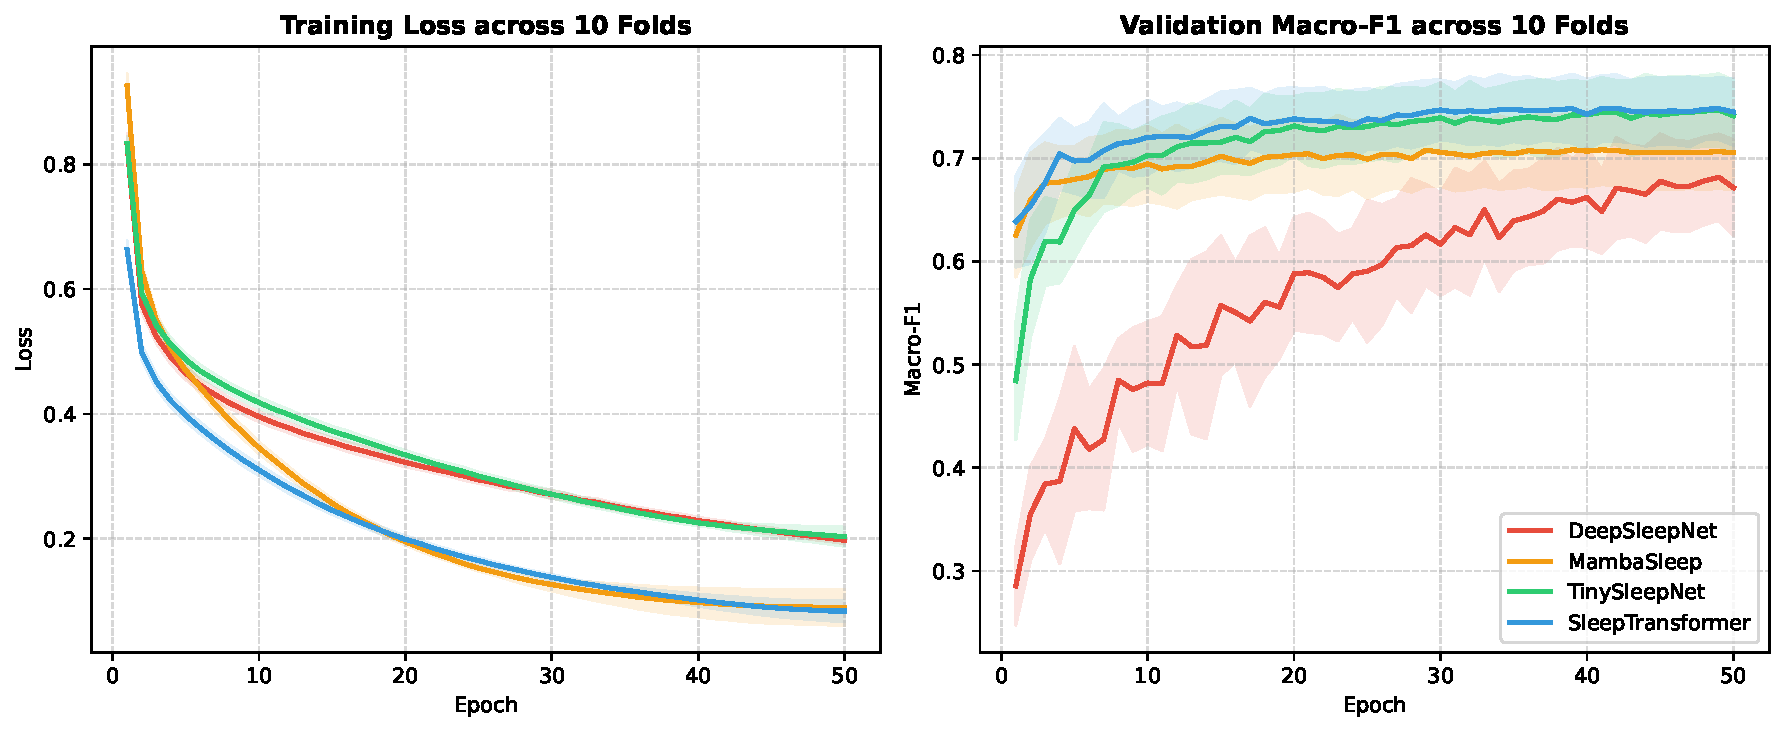
\includegraphics[width=0.5\textwidth]{learning_curves.pdf}
\caption{Aggregated training curves across all ten cross-validation folds for TinySleepNet-adapted, DeepSleepNet-adapted, SleepTransformer-adapted, and MambaSleep-adapted. The solid lines represent the mean training loss (left) and validation macro-F1 score (right) over 50 epochs, while the shaded regions denote the standard deviation across the ten folds.}
\label{fig:learning_curves}
\end{figure}

Fig.~\ref{fig:learning_curves} illustrates the aggregated learning curves for the four evaluated architectures. TinySleepNet-adapted and SleepTransformer-adapted converged rapidly, reaching stable performance near $0.74$ within 20 epochs on validation macro-F1. DeepSleepNet-adapted exhibited slow convergence and substantial variation across different subject-wise validation folds, which reflects the difficulty of training the deeper dual-branch CNN--BiLSTM architecture in a single end-to-end stage without two-stage optimization. SleepTransformer-adapted and MambaSleep-adapted achieved lower final training losses (below $0.10$) than TinySleepNet-adapted and DeepSleepNet-adapted (approximately $0.20$), suggesting that they fitted the training data more closely under the present optimization protocol. MambaSleep-adapted converged to a slightly lower validation macro-F1 ($0.70$) and showed a relatively narrow standard-deviation band across folds. This pattern indicates lower observed cross-fold variation under the present protocol, but it should not be interpreted as evidence of intrinsic architectural stability because each fold involved different subjects and only one training run was performed per fold.

In terms of observed training time, TinySleepNet-adapted required
$105.8 \pm 10.8$ minutes per fold on average, with $134.0 \pm 3.0$
s/epoch and an average of $47.4$ trained epochs. DeepSleepNet-adapted
required $127.5 \pm 3.2$ minutes per fold, with $150.6 \pm 3.5$
s/epoch and an average of $50.8$ epochs, whereas SleepTransformer-adapted
required $129.3 \pm 15.7$ minutes per fold, with $165.1 \pm 2.0$
s/epoch and an average of $47.0$ epochs. MambaSleep-adapted had the
lowest observed per-epoch training time at $121.8 \pm 2.8$ s/epoch and
required $83.4 \pm 17.1$ minutes per fold while training for an
average of $41.0$ epochs. The lower per-epoch time suggests reduced
computational cost under the present implementation and hardware
configuration. However, its lower total fold duration was also
influenced by earlier stopping. Therefore, total training time per
fold should not be interpreted as a purely architectural efficiency
measure.

\subsection{Class-Wise Performance}

\begin{table}[h]
\centering
\caption{Class-Wise F1 Across Ten Test Folds. All architectures represent adapted implementations evaluated under the proposed unified framework.}
\label{tab:classwise}
\resizebox{\columnwidth}{!}{
\begin{tabular}{lcccc}
\toprule
Class & TinySleepNet-adapted & DeepSleepNet-adapted & SleepTransformer-adapted & MambaSleep-adapted \\
\midrule
W &
$0.9678\pm0.0091$ &
$0.9186\pm0.0341$ &
$\mathbf{0.9737\pm0.0063}$ &
$0.9687\pm0.0086$ \\
N1 &
$0.4664\pm0.0520$ &
$0.3499\pm0.0590$ &
$\mathbf{0.4790\pm0.0518}$ &
$0.4252\pm0.0378$ \\
N2 &
$0.8007\pm0.0406$ &
$0.7815\pm0.0408$ &
$\mathbf{0.8099\pm0.0302}$ &
$0.7834\pm0.0283$ \\
N3 &
$0.7026\pm0.0695$ &
$0.6775\pm0.1079$ &
$\mathbf{0.7134\pm0.0574}$ &
$0.6713\pm0.0617$ \\
REM &
$0.7821\pm0.0514$ &
$0.6839\pm0.0827$ &
$\mathbf{0.7851\pm0.0393}$ &
$0.6968\pm0.0608$ \\
\bottomrule
\end{tabular}}
\end{table}


TinySleepNet-adapted achieved competitive stage F1 scores, particularly for REM and N1. DeepSleepNet-adapted obtained the lowest F1 values across all stages. SleepTransformer-adapted obtained the highest mean F1 for every stage, although TinySleepNet-adapted was close for REM and N1. MambaSleep-adapted performed moderately across stages. Wake was the easiest stage for all architectures, consistent with both its strong signal distinction and its dominant representation in the corpus.

\begin{figure*}[t]
\centering
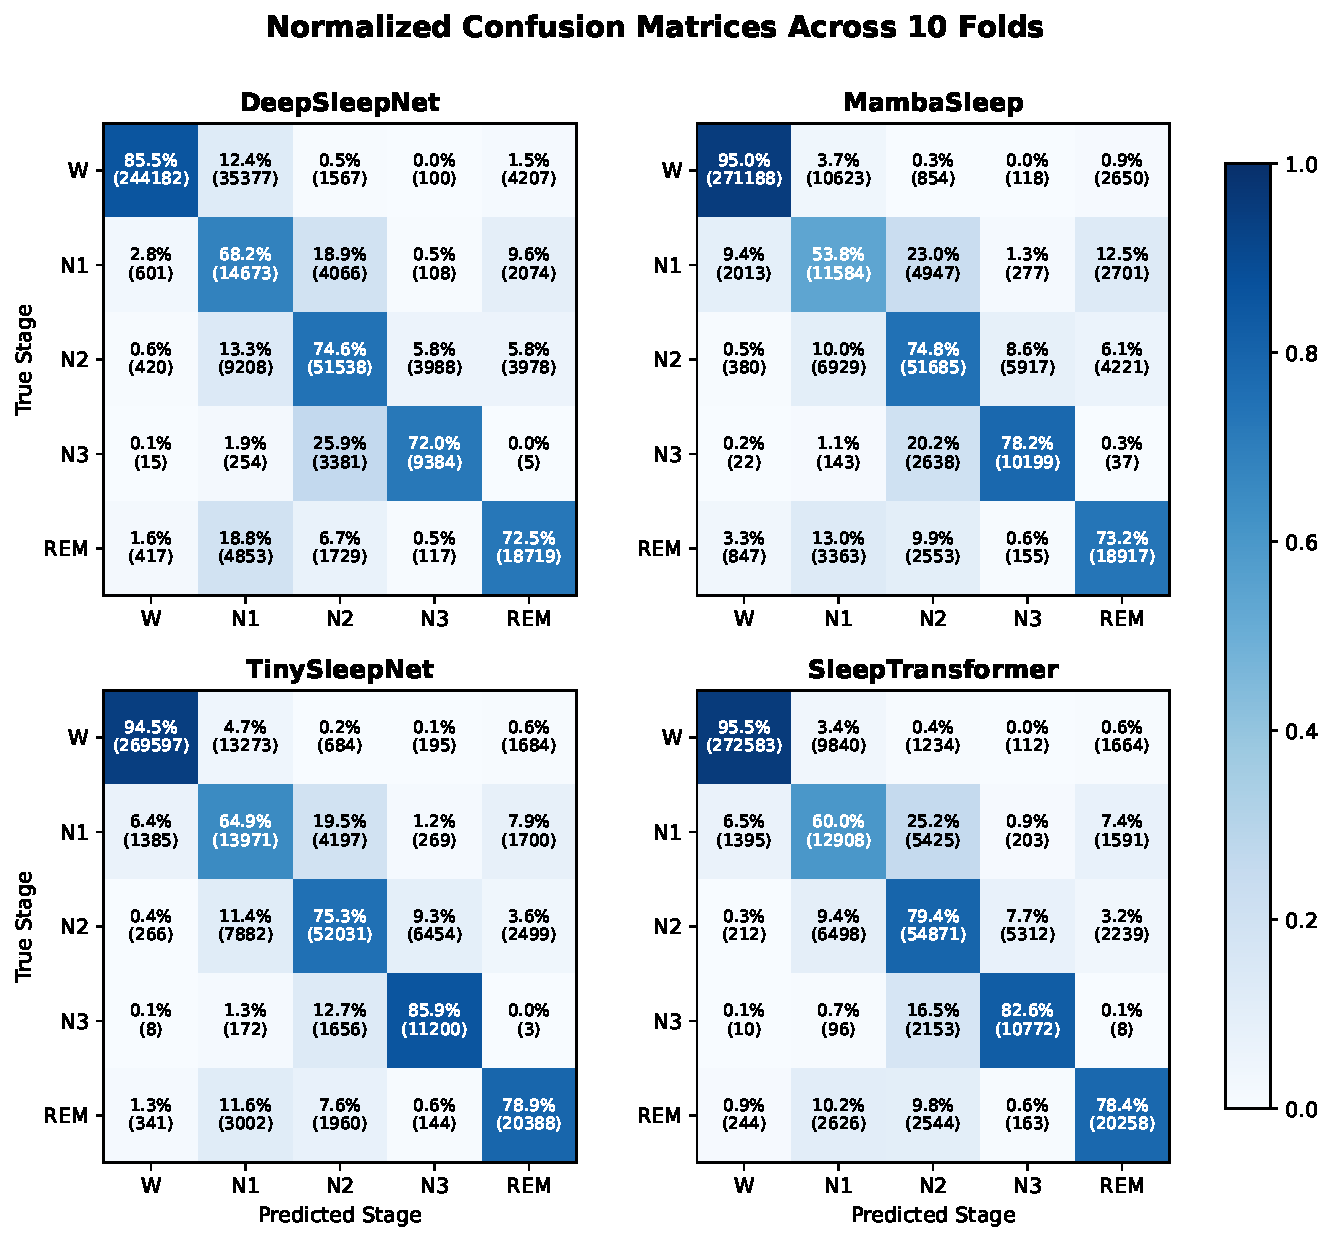
\includegraphics[width=0.85\textwidth]{confusion_matrices.pdf}
\caption{Normalized Confusion Matrices across all ten cross-validation folds for TinySleepNet-adapted, DeepSleepNet-adapted, SleepTransformer-adapted, and MambaSleep-adapted. Values inside each cell represent the percentage of true sleep stages (recall) and the absolute epoch counts in parentheses.}
\label{fig:confusion_matrices}
\end{figure*}


N1 was the most difficult stage for every architecture, with F1 values from 0.3499 to 0.4790. Importantly, N1 was not the smallest class: N3 contained 13,039 epochs compared with 21,522 N1 epochs. N3 nevertheless achieved substantially higher F1. This finding indicates that N1 difficulty is not explained by frequency alone and is consistent with its transitional characteristics and overlap with Wake, N2, and REM.

The consolidated confusion matrices in Fig.~\ref{fig:confusion_matrices} highlight the specific misclassifications driving these class-wise patterns. Across all four architectures, True N1 epochs are frequently misclassified as N2 ($19.5\%$ for TinySleepNet-adapted, $18.9\%$ for DeepSleepNet-adapted, $25.2\%$ for SleepTransformer-adapted, and $23.0\%$ for MambaSleep-adapted), reflecting the physiological transition where transitional slow-wave activity begins to merge with sleep spindles and K-complexes. True N1 is also commonly misclassified as Wake ($6.4\%$, $2.8\%$, $6.5\%$, and $9.4\%$, respectively) or REM ($7.9\%$, $9.6\%$, $7.4\%$, and $12.5\%$, respectively). Furthermore, True REM epochs are frequently misclassified as N1 ($11.6\%$ for TinySleepNet-adapted and $10.2\%$ for SleepTransformer-adapted) because they share low-voltage, mixed-frequency EEG background characteristics. Class-weighted loss improved the training objective but did not eliminate the minority-stage problem, which has also motivated specialized imbalance methods in prior work \cite{zhou2022imbalance}.

\subsection{Variation Across Subject-Wise Folds}

TinySleepNet-adapted showed moderate standard deviation across the ten subject-wise test folds. DeepSleepNet-adapted showed the largest variation, particularly for Cohen's kappa and N3 F1. SleepTransformer-adapted had the lowest observed standard deviation for accuracy, macro-F1, and Cohen's kappa. MambaSleep-adapted had the second-lowest cross-fold variation for the three overall metrics, although its mean macro-F1 was lower than that of TinySleepNet-adapted.

These standard deviations should not be interpreted as direct estimates of training repeatability or intrinsic model stability. Each fold contained a different group of held-out subjects, and each architecture was trained only once per fold. Consequently, the observed variation combines differences in subject composition, training data composition, model initialization, augmentation, and optimization. Repeated training with multiple seeds on each fold would be required to separate variation caused by subject selection from variation caused by stochastic training.

\section{Discussion}

\begin{table*}[t]
\centering
\caption{Comparison between reported performance of original architectures and our adapted implementations. The original reported results are included for contextual reference only and do not represent direct reproduction results from this study. Adapted implementations are not exact reproductions of the original architectures.}
\label{tab:contextual_comparison}
\centering
\begin{tabular}{lllp{2.5cm}ll}
\toprule
Architecture & Implementation & Dataset / EEG Channel & Validation Protocol & Reported Result  \\
\midrule
\multirow{2}{*}{\begin{tabular}[c]{@{}l@{}}TinySleepNet-adapted\\ (based on TinySleepNet)\end{tabular}} & Original \cite{supratak2020tinysleepnet} & Sleep-EDF (78 sub.), Fpz--Cz & subject-wise 10-fold & 83.1\% ACC, 78.1\% MF1  \\
& Our adapted implementation & Sleep-EDF (78 sub.), Fpz--Cz & subject-wise 10-fold & 88.48\% ACC, 74.39\% MF1  \\
\midrule
\multirow{2}{*}{\begin{tabular}[c]{@{}l@{}}DeepSleepNet-adapted\\ (based on DeepSleepNet)\end{tabular}} & Original two-stage \cite{supratak2017deepsleepnet} & Sleep-EDF (20 sub.), Fpz--Cz & subject-wise 20-fold & 82.0\% ACC, 76.9\% MF1  \\
& Our adapted implementation & Sleep-EDF (78 sub.), Fpz--Cz & subject-wise 10-fold & 81.59\% ACC, 68.23\% MF1  \\
\midrule
\multirow{3}{*}{\begin{tabular}[c]{@{}l@{}}SleepTransformer-adapted\\ (based on SleepTransformer)\end{tabular}} & Original scratch \cite{phan2022sleeptransformer} & Sleep-EDF (78 sub.), Fpz--Cz & subject-wise 10-fold & 81.4\% ACC, 74.3\% MF1  \\
& Original fine-tuned (SHHS) \cite{phan2022sleeptransformer} & Sleep-EDF (78 sub.), Fpz--Cz & subject-wise 10-fold & 84.9\% ACC, 78.8\% MF1  \\
& Our adapted implementation & Sleep-EDF (78 sub.), Fpz--Cz & subject-wise 10-fold & 89.51\% ACC, 75.22\% MF1  \\
\midrule
\multirow{2}{*}{\begin{tabular}[c]{@{}l@{}}MambaSleep-adapted\\ (based on Mamba architecture)\end{tabular}} & Original WaveMamba full-night \cite{sano2025wavemamba} & Sleep-EDF (78 sub.), Fpz--Cz & subject-wise 10-fold & 86.0\% ACC, 78.6\% MF1 \\
& Our adapted implementation & Sleep-EDF (78 sub.), Fpz--Cz &  subject-wise 10-fold  & 87.61\% ACC, 70.91\% MF1  \\
\bottomrule
\end{tabular}
\end{table*}



The benchmark produced three main findings. First, TinySleepNet-adapted remains a strong baseline despite its simpler recurrent architecture; its performance is competitive and only the accuracy difference was found to be statistically significant after correction. DeepSleepNet-adapted demonstrated the lowest observed metrics under this end-to-end training setup. SleepTransformer-adapted achieved the strongest observed overall performance, though its macro-F1 and Cohen's kappa advantages over TinySleepNet-adapted did not establish a statistically significant separation in the exploratory comparisons. Finally, MambaSleep-adapted achieved moderate results, exceeding DeepSleepNet-adapted but not matching the other architectures.

To provide historical context, Table~\ref{tab:contextual_comparison} compiles the results reported in the original publications alongside the results obtained in this study. We emphasize that this is a contextual reference rather than a direct, head-to-head comparison. The published values were obtained under differing conditions including exact database split protocols, preprocessing choices, wake-trimming rules, EEG derivations, input context lengths, and network implementations. For instance, our repository-based TinySleepNet-adapted and raw-EEG SleepTransformer-adapted achieved higher observed performance in this specific subject-wise benchmark than reported in their original publications, which likely reflects the specific preprocessing and sequence construction parameters used in our evaluation pipeline. Conversely, the original DeepSleepNet model was trained using a two-stage optimization process, whereas DeepSleepNet-adapted is trained end-to-end in one stage. For the state-space approach, WaveMamba (used as a literature reference for full-night Mamba staging) was designed for full-night or 200-epoch sequence processing, and its performance degrades under the lightweight, 20-epoch sequence configuration evaluated in MambaSleep-adapted. WaveMamba results are derived from a recent preprint and should therefore be interpreted accordingly.

Second, the lightweight MambaSleep-adapted architecture improved accuracy and Cohen's kappa relative to the DeepSleepNet-adapted implementation, while macro-F1 showed numerical improvement without reaching statistical significance. However, it did not surpass TinySleepNet-adapted or SleepTransformer-adapted. The result should not be interpreted as a general rejection of state-space modeling. The implementation scans only 20 epochs and simplifies the computational structure by avoiding expensive Mamba stacks in the frequency branches. These choices improve practicality but reduce the full-night, long-context advantage of full-night models like WaveMamba. An evaluation with longer contexts and a closer architectural reproduction would be required for a broader conclusion.

Third, N1 remained the principal class-level limitation. N3 was less frequent yet substantially easier to recognize, indicating that stage ambiguity matters in addition to imbalance. N1 often occupies transitions and can share characteristics with neighboring stages. Future work could evaluate transition-aware objectives, calibrated uncertainty, focal or margin-based losses, targeted augmentation, and post-processing with physiologically plausible transition constraints. Relevant work on attention, explainability, and imbalance provides several directions \cite{eldele2021attention,dutt2023sleepxai,zhou2022imbalance}.

The full-recording preprocessing used here also affects interpretation. Because no wake trimming was applied, Wake represents 68.79\% of the corpus. Accuracy is therefore influenced heavily by Wake performance, which makes macro-F1 essential for comparing balanced stage recognition. The per-epoch Z-score normalization standardizes amplitude independently in each epoch and may improve numerical stability, but it can also remove between-epoch amplitude information. These are properties of the evaluated corpus rather than universal preprocessing recommendations.

The study has several limitations. The statistical sensitivity is limited by the number of subject-level folds, and significance results should therefore be interpreted cautiously. Only one database and one EEG derivation were evaluated, so cross-dataset and cross-device generalization remain unknown. Each model was trained once per fold using one seeded execution; robustness across repeated random initializations was not measured. The four systems are repository adaptations with unequal fidelity to their source papers. No standardized parameter-count, inference-latency, memory, or energy benchmark was performed. The 20-epoch context may disadvantage methods intended for full-night modeling. Finally, the study does not evaluate interpretability, uncertainty calibration, transfer learning, self-supervised pretraining, personalization, or domain adaptation, despite their importance in prior work \cite{phan2020personalized,phan2020transfer,fan2022domain,eldele2023selfsupervised}.

\section{Conclusion}

This study presented a unified subject-wise evaluation of adapted CNN-based, CNN-RNN, Transformer-based, and State Space architectures for single-channel EEG sleep staging. The preprocessing description was grounded in the project notebook: 30-s epochs at 100 Hz, stage-3/stage-4 merging, exclusion of non-target annotations, independent epoch-wise Z-score normalization, and NPZ storage without additional filtering or wake trimming.

Under a shared 10-fold protocol, TinySleepNet-adapted remained statistically close in macro-F1 and Cohen's kappa, showing that a compact CNN--LSTM can be highly competitive. DeepSleepNet-adapted showed the lowest observed metrics. SleepTransformer-adapted achieved the highest observed means for accuracy, macro-F1, Cohen's kappa, and all five class-wise F1 scores. MambaSleep-adapted demonstrated numerical improvement over DeepSleepNet-adapted but did not match SleepTransformer-adapted or TinySleepNet-adapted under the 20-epoch setting. N1 remained the central class-level challenge even though N3 was less frequent.

Future work should evaluate repeated seeds, external datasets, longer temporal contexts, standardized efficiency measurements, and ablations of preprocessing, augmentation, class weighting, wavelet decomposition, attention, and temporal state-space blocks. Such experiments would separate architectural effects from implementation and protocol effects more reliably.

\section{Code Availability}

The benchmark implementation and fold-level results are available at:
\url{https://github.com/baodeptraivcll/SLEEP}.


\bibliographystyle{IEEEtran}
\bibliography{references}

\end{document}
